\chapter{Praktická část}


\section{Výběr úloh}

Nejdříve jsme získali přijímací zkoušky CERMAT od roku 2015 do roku 2022. Ty jsou volně dostupné na internetu. Z každého roku jsme se snažili čerpat z~pravých testů, tedy řádných a náhradních termínů, a ne ilustračních. Pokud ale v daný rok bylo pravých testů málo, použili jsme i ty.

Jako první jsme tyto zkoušky prošli, a vybrali z nich všechny úlohy které se týkají planimetrie nebo stereometrie.

Následovně jsme tyto úlohy kategorizovali podle
\begin{itemize}
    \item typu oboru,
    \item termínu ze kterého pochází
    \item a posledně do 3 hlavních kategorií, jimiž jsou
    \begin{itemize}
        \item úlohy planimetrické,
        \item stereometrické a
        \item rýsovací.
    \end{itemize}
\end{itemize}

V testech se neobjevily žádné stereometrické rýsovací úlohy, pouze planimetrické rýsovací.

Úloh jsme napříč vybrali 456.

Následně jsme všechny úlohy jednoho oboru dali k sobě podle kategorií a~vytvořili podkategorie. Například jedna z podkategorií planimetrických úloh pro 6leté obory byly úlohy zaměřené na úhly.


\section[Statistická analýza přijímacích zkoušek z minulých let]{Statistická analýza přijímacích zkoušek\\z minulých let}

Po roztřídění všech úloh jsme spočítali, jak často se v testech objevují a jakou mají bodovou váhu.

Přišli jsme k závěru že planimetrické a stereometrické úlohy jsou velmi důležité, jelikož v 8letých oborech odpovídají skoro 38 \% známky. Také se planimetrické, rýsovací a stereometrické úlohy objevují přibližně v poměru 2 : 1 : 1 pro tyto obory.

\begin{table}[htbp]
    \caption{Distribuce počtu úloh pro 8leté obory}
    \begin{tabular}{|l|l|r|r|r|r|}
        \hline
        \multicolumn{ 2}{|c|}{8leté obory} & \multicolumn{ 4}{c|}{Počet úloh} \\ \cline{ 3- 6}
        \multicolumn{ 2}{|l|}{} & \multicolumn{1}{c|}{Planimetrie} & \multicolumn{1}{c|}{\begin{tabular}[c]{@{}c@{}}
                                                                                             Rýsování\\ planimetrie
        \end{tabular}} & \multicolumn{1}{c|}{Stereometrie} & \multicolumn{1}{c|}{Celkem} \\ \hline
        \multicolumn{ 1}{|c|}{2022} & 1. řádný termín    & 2 & 1 & 1 & 14 \\ \cline{ 2- 6}
        \multicolumn{ 1}{|l|}{}     & 2. řádný termín    & 1 & 1 & 3 & 14 \\ \cline{ 2- 6}
        \multicolumn{ 1}{|l|}{}     & 1. náhradní termín & 4 & 1 & 1 & 14 \\ \cline{ 2- 6}
        \multicolumn{ 1}{|l|}{}     & 2. náhradní termín & 2 & 1 & 2 & 14 \\ \hline
        \multicolumn{ 1}{|c|}{2021} & 1. řádný termín    & 2 & 1 & 1 & 14 \\ \cline{ 2- 6}
        \multicolumn{ 1}{|l|}{}     & 2. řádný termín    & 2 & 1 & 1 & 14 \\ \cline{ 2- 6}
        \multicolumn{ 1}{|l|}{}     & 1. náhradní termín & 3 & 1 & 1 & 14 \\ \cline{ 2- 6}
        \multicolumn{ 1}{|l|}{}     & 2. náhradní termín & 2 & 1 & 1 & 14 \\ \hline
        \multicolumn{ 1}{|c|}{2020} & 1. řádný termín    & 2 & 1 & 1 & 14 \\ \cline{ 2- 6}
        \multicolumn{ 1}{|l|}{}     & 1. náhradní termín & 3 & 1 & 1 & 14 \\ \hline
        \multicolumn{ 1}{|c|}{2019} & 1. řádný termín    & 3 & 1 & 1 & 14 \\ \cline{ 2- 6}
        \multicolumn{ 1}{|l|}{}     & 2. řádný termín    & 3 & 1 & 1 & 14 \\ \cline{ 2- 6}
        \multicolumn{ 1}{|l|}{}     & 1. náhradní termín & 2 & 1 & 2 & 14 \\ \cline{ 2- 6}
        \multicolumn{ 1}{|l|}{}     & 2. náhradní termín & 1 & 1 & 2 & 14 \\ \hline
        \multicolumn{ 1}{|c|}{2018} & 1. řádný termín    & 1 & 1 & 1 & 14 \\ \cline{ 2- 6}
        \multicolumn{ 1}{|l|}{}     & 2. řádný termín    & 2 & 1 & 2 & 14 \\ \cline{ 2- 6}
        \multicolumn{ 1}{|l|}{}     & 1. náhradní termín & 1 & 1 & 2 & 14 \\ \cline{ 2- 6}
        \multicolumn{ 1}{|l|}{}     & 2. náhradní termín & 4 & 1 & 1 & 14 \\ \hline
        \multicolumn{ 1}{|c|}{2017} & 1. řádný termín    & 1 & 1 & 1 & 14 \\ \cline{ 2- 6}
        \multicolumn{ 1}{|l|}{}     & 2. řádný termín    & 3 & 1 & 1 & 14 \\ \cline{ 2- 6}
        \multicolumn{ 1}{|l|}{}     & 1. náhradní termín & 3 & 1 & 1 & 14 \\ \cline{ 2- 6}
        \multicolumn{ 1}{|l|}{}     & 2. náhradní termín & 3 & 1 & 1 & 14 \\ \hline
        \multicolumn{ 1}{|c|}{2016} & 1. řádný termín    & 3 & 1 & 2 & 16 \\ \cline{ 2- 6}
        \multicolumn{ 1}{|l|}{}     & Ilustrační         & 3 & 1 & 2 & 16 \\ \hline
        \multicolumn{ 1}{|c|}{2015} & 1. řádný termín    & 2 & 1 & 2 & 16 \\ \cline{ 2- 6}
        \multicolumn{ 1}{|l|}{}     & Ilustrační         & 2 & 2 & 1 & 17 \\ \hline
        \multicolumn{ 2}{|c|}{Průměr} & 2,31 & 1,04 & 1,38 & 14,35 \\ \hline
        \multicolumn{ 2}{|c|}{Průměrná četnost} & 16,09 \% & 7,24 \% & 9,65 \% & 32,98 \% \\ \hline
    \end{tabular}
    \label{tabulka8-1}
\end{table}

\begin{table}[htbp]
    \caption{Distribuce bodů za úlohu pro 8leté obory}
    \begin{tabular}{|l|l|r|r|r|r|}
        \hline
        \multicolumn{ 2}{|c|}{8leté obory} & \multicolumn{ 4}{c|}{Body za úlohy} \\ \cline{ 3- 6}
        \multicolumn{ 2}{|l|}{} & \multicolumn{1}{c|}{Planimetrie} & \multicolumn{1}{c|}{\begin{tabular}[c]{@{}c@{}}
                                                                                             Rýsování\\ planimetrie
        \end{tabular}} & \multicolumn{1}{c|}{Stereometrie} & \multicolumn{1}{c|}{Celkem} \\ \hline
        \multicolumn{ 1}{|c|}{2022} & 1. řádný termín    & 8  & 6 & 5 & 50 \\ \cline{ 2- 6}
        \multicolumn{ 1}{|l|}{}     & 2. řádný termín    & 2  & 6 & 7 & 50 \\ \cline{ 2- 6}
        \multicolumn{ 1}{|l|}{}     & 1. náhradní termín & 10 & 6 & 5 & 50 \\ \cline{ 2- 6}
        \multicolumn{ 1}{|l|}{}     & 2. náhradní termín & 12 & 6 & 4 & 50 \\ \hline
        \multicolumn{ 1}{|c|}{2021} & 1. řádný termín    & 8  & 6 & 5 & 50 \\ \cline{ 2- 6}
        \multicolumn{ 1}{|l|}{}     & 2. řádný termín    & 6  & 6 & 5 & 50 \\ \cline{ 2- 6}
        \multicolumn{ 1}{|l|}{}     & 1. náhradní termín & 10 & 6 & 5 & 50 \\ \cline{ 2- 6}
        \multicolumn{ 1}{|l|}{}     & 2. náhradní termín & 8  & 6 & 2 & 50 \\ \hline
        \multicolumn{ 1}{|c|}{2020} & 1. řádný termín    & 8  & 6 & 5 & 50 \\ \cline{ 2- 6}
        \multicolumn{ 1}{|l|}{}     & 1. náhradní termín & 12 & 6 & 4 & 50 \\ \hline
        \multicolumn{ 1}{|c|}{2019} & 1. řádný termín    & 12 & 6 & 5 & 50 \\ \cline{ 2- 6}
        \multicolumn{ 1}{|l|}{}     & 2. řádný termín    & 12 & 6 & 5 & 50 \\ \cline{ 2- 6}
        \multicolumn{ 1}{|l|}{}     & 1. náhradní termín & 8  & 6 & 4 & 50 \\ \cline{ 2- 6}
        \multicolumn{ 1}{|l|}{}     & 2. náhradní termín & 4  & 6 & 4 & 50 \\ \hline
        \multicolumn{ 1}{|c|}{2018} & 1. řádný termín    & 4  & 6 & 5 & 50 \\ \cline{ 2- 6}
        \multicolumn{ 1}{|l|}{}     & 2. řádný termín    & 8  & 6 & 4 & 50 \\ \cline{ 2- 6}
        \multicolumn{ 1}{|l|}{}     & 1. náhradní termín & 4  & 6 & 4 & 50 \\ \cline{ 2- 6}
        \multicolumn{ 1}{|l|}{}     & 2. náhradní termín & 12 & 6 & 2 & 50 \\ \hline
        \multicolumn{ 1}{|c|}{2017} & 1. řádný termín    & 4  & 6 & 5 & 50 \\ \cline{ 2- 6}
        \multicolumn{ 1}{|l|}{}     & 2. řádný termín    & 8  & 6 & 5 & 50 \\ \cline{ 2- 6}
        \multicolumn{ 1}{|l|}{}     & 1. náhradní termín & 11 & 6 & 2 & 50 \\ \cline{ 2- 6}
        \multicolumn{ 1}{|l|}{}     & 2. náhradní termín & 11 & 6 & 2 & 50 \\ \hline
        \multicolumn{ 1}{|c|}{2016} & 1. řádný termín    & 10 & 6 & 4 & 50 \\ \cline{ 2- 6}
        \multicolumn{ 1}{|l|}{}     & Ilustrační         & 10 & 6 & 4 & 50 \\ \hline
        \multicolumn{ 1}{|c|}{2015} & 1. řádný termín    & 6  & 6 & 4 & 50 \\ \cline{ 2- 6}
        \multicolumn{ 1}{|l|}{}     & Ilustrační         & 6  & 8 & 6 & 50 \\ \hline
        \multicolumn{ 2}{|c|}{Průměr} & 8,23 & 6,08 & 4,31 & 50,00 \\ \hline
        \multicolumn{ 2}{|c|}{\begin{tabular}[c]{@{}c@{}}
                                  Průměrná\\ četnost
        \end{tabular}} & 16,46 \% & 12,15 \% & 8,62 \% & 37,23 \% \\ \hline
    \end{tabular}
    \label{tabulka8-2}
\end{table}


\begin{table}[htbp]
    \caption{Distribuce počtu úloh pro 6leté obory}
    \begin{tabular}{|l|l|r|r|r|r|}
        \hline
        \multicolumn{ 2}{|l|}{6leté obory} & \multicolumn{ 3}{c|}{Počet úloh co obsahuje} & \multicolumn{ 1}{c|}{Celkem} \\ \cline{ 3- 5}
        \multicolumn{ 2}{|l|}{} & \multicolumn{1}{c|}{Planimetrie} & \multicolumn{1}{c|}{\begin{tabular}[c]{@{}c@{}}
                                                                                             Rýsování\\ planimetrie
        \end{tabular}} & \multicolumn{1}{c|}{Stereometrie} & \multicolumn{ 1}{c|}{} \\ \hline
        \multicolumn{ 1}{|c|}{2022} & 1. řádný termín    & 4 & 2 & 0 & 16 \\ \cline{ 2- 6}
        \multicolumn{ 1}{|l|}{}     & 2. řádný termín    & 4 & 2 & 1 & 16 \\ \cline{ 2- 6}
        \multicolumn{ 1}{|l|}{}     & 1. náhradní termín & 6 & 2 & 0 & 16 \\ \cline{ 2- 6}
        \multicolumn{ 1}{|l|}{}     & 2. náhradní termín & 3 & 2 & 1 & 16 \\ \hline
        \multicolumn{ 1}{|c|}{2021} & 1. řádný termín    & 3 & 2 & 1 & 16 \\ \cline{ 2- 6}
        \multicolumn{ 1}{|l|}{}     & 2. řádný termín    & 2 & 2 & 2 & 16 \\ \cline{ 2- 6}
        \multicolumn{ 1}{|l|}{}     & 1. náhradní termín & 4 & 2 & 1 & 16 \\ \cline{ 2- 6}
        \multicolumn{ 1}{|l|}{}     & 2. náhradní termín & 4 & 2 & 1 & 16 \\ \hline
        \multicolumn{ 1}{|c|}{2020} & 1. řádný termín    & 3 & 2 & 1 & 16 \\ \cline{ 2- 6}
        \multicolumn{ 1}{|l|}{}     & 1. náhradní termín & 3 & 2 & 1 & 16 \\ \hline
        \multicolumn{ 1}{|c|}{2019} & 1. řádný termín    & 3 & 2 & 1 & 16 \\ \cline{ 2- 6}
        \multicolumn{ 1}{|l|}{}     & 2. řádný termín    & 3 & 2 & 1 & 16 \\ \cline{ 2- 6}
        \multicolumn{ 1}{|l|}{}     & 1. náhradní termín & 5 & 2 & 0 & 16 \\ \cline{ 2- 6}
        \multicolumn{ 1}{|l|}{}     & 2. náhradní termín & 3 & 1 & 1 & 16 \\ \hline
        \multicolumn{ 1}{|c|}{2018} & 1. řádný termín    & 3 & 2 & 0 & 16 \\ \cline{ 2- 6}
        \multicolumn{ 1}{|l|}{}     & 2. řádný termín    & 3 & 2 & 1 & 16 \\ \cline{ 2- 6}
        \multicolumn{ 1}{|l|}{}     & 1. náhradní termín & 3 & 2 & 0 & 16 \\ \cline{ 2- 6}
        \multicolumn{ 1}{|l|}{}     & 2. náhradní termín & 3 & 2 & 1 & 16 \\ \hline
        \multicolumn{ 1}{|c|}{2017} & 1. řádný termín    & 3 & 2 & 1 & 17 \\ \cline{ 2- 6}
        \multicolumn{ 1}{|l|}{}     & 2. řádný termín    & 4 & 2 & 1 & 17 \\ \cline{ 2- 6}
        \multicolumn{ 1}{|l|}{}     & 1. náhradní termín & 4 & 2 & 2 & 17 \\ \cline{ 2- 6}
        \multicolumn{ 1}{|l|}{}     & 2. náhradní termín & 4 & 2 & 0 & 17 \\ \hline
        \multicolumn{ 1}{|c|}{2016} & 1. řádný termín    & 3 & 1 & 1 & 17 \\ \cline{ 2- 6}
        \multicolumn{ 1}{|l|}{}     & Ilustrační         & 4 & 1 & 1 & 17 \\ \hline
        \multicolumn{ 1}{|c|}{2015} & 1. řádný termín    & 3 & 1 & 1 & 17 \\ \cline{ 2- 6}
        \multicolumn{ 1}{|l|}{}     & Ilustrační         & 2 & 2 & 2 & 17 \\ \hline
        \multicolumn{ 2}{|c|}{Průměr} & 3,42 & 1,85 & 0,88 & 16,31 \\ \hline
        \multicolumn{ 2}{|c|}{Průměrná četnost} & 20,99 \% & 11,32 \% & 5,42 \% & 37,74 \% \\ \hline
    \end{tabular}
    \label{tabulka6-1}
\end{table}

\begin{table}[htbp]
    \caption{Distribuce bodů za úlohu pro 6leté obory}
    \begin{tabular}{|l|l|r|r|r|r|}
        \hline
        \multicolumn{ 2}{|l|}{6leté obory} & \multicolumn{ 3}{c|}{Celkem bodů} & \multicolumn{ 1}{c|}{Celkem} \\ \cline{ 3- 5}
        \multicolumn{ 2}{|l|}{} & \multicolumn{1}{c|}{Planimetrie} & \multicolumn{1}{c|}{\begin{tabular}[c]{@{}c@{}}
                                                                                             Rýsování\\ planimetrie
        \end{tabular}} & \multicolumn{1}{c|}{Stereometrie} & \multicolumn{ 1}{c|}{} \\ \hline
        \multicolumn{ 1}{|c|}{2022} & 1. řádný termín    & 8  & 6 & 2 & 50 \\ \cline{ 2- 6}
        \multicolumn{ 1}{|l|}{}     & 2. řádný termín    & 10 & 6 & 4 & 50 \\ \cline{ 2- 6}
        \multicolumn{ 1}{|l|}{}     & 1. náhradní termín & 13 & 6 & 4 & 50 \\ \cline{ 2- 6}
        \multicolumn{ 1}{|l|}{}     & 2. náhradní termín & 9  & 6 & 2 & 50 \\ \hline
        \multicolumn{ 1}{|c|}{2021} & 1. řádný termín    & 10 & 6 & 4 & 50 \\ \cline{ 2- 6}
        \multicolumn{ 1}{|l|}{}     & 2. řádný termín    & 5  & 6 & 4 & 50 \\ \cline{ 2- 6}
        \multicolumn{ 1}{|l|}{}     & 1. náhradní termín & 14 & 6 & 2 & 50 \\ \cline{ 2- 6}
        \multicolumn{ 1}{|l|}{}     & 2. náhradní termín & 12 & 6 & 2 & 50 \\ \hline
        \multicolumn{ 1}{|c|}{2020} & 1. řádný termín    & 10 & 6 & 4 & 50 \\ \cline{ 2- 6}
        \multicolumn{ 1}{|l|}{}     & 1. náhradní termín & 10 & 6 & 4 & 50 \\ \hline
        \multicolumn{ 1}{|c|}{2019} & 1. řádný termín    & 10 & 5 & 4 & 50 \\ \cline{ 2- 6}
        \multicolumn{ 1}{|l|}{}     & 2. řádný termín    & 10 & 5 & 3 & 50 \\ \cline{ 2- 6}
        \multicolumn{ 1}{|l|}{}     & 1. náhradní termín & 14 & 5 & 4 & 50 \\ \cline{ 2- 6}
        \multicolumn{ 1}{|l|}{}     & 2. náhradní termín & 6  & 5 & 3 & 50 \\ \hline
        \multicolumn{ 1}{|c|}{2018} & 1. řádný termín    & 10 & 6 & 0 & 50 \\ \cline{ 2- 6}
        \multicolumn{ 1}{|l|}{}     & 2. řádný termín    & 10 & 6 & 4 & 50 \\ \cline{ 2- 6}
        \multicolumn{ 1}{|l|}{}     & 1. náhradní termín & 8  & 6 & 0 & 50 \\ \cline{ 2- 6}
        \multicolumn{ 1}{|l|}{}     & 2. náhradní termín & 9  & 6 & 2 & 50 \\ \hline
        \multicolumn{ 1}{|c|}{2017} & 1. řádný termín    & 8  & 6 & 3 & 50 \\ \cline{ 2- 6}
        \multicolumn{ 1}{|l|}{}     & 2. řádný termín    & 12 & 6 & 3 & 50 \\ \cline{ 2- 6}
        \multicolumn{ 1}{|l|}{}     & 1. náhradní termín & 12 & 6 & 4 & 50 \\ \cline{ 2- 6}
        \multicolumn{ 1}{|l|}{}     & 2. náhradní termín & 11 & 5 & 2 & 50 \\ \hline
        \multicolumn{ 1}{|c|}{2016} & 1. řádný termín    & 9  & 5 & 3 & 50 \\ \cline{ 2- 6}
        \multicolumn{ 1}{|l|}{}     & Ilustrační         & 10 & 6 & 2 & 50 \\ \hline
        \multicolumn{ 1}{|c|}{2015} & 1. řádný termín    & 7  & 6 & 2 & 50 \\ \cline{ 2- 6}
        \multicolumn{ 1}{|l|}{}     & Ilustrační         & 5  & 5 & 5 & 50 \\ \hline
        \multicolumn{ 2}{|c|}{Průměr} & 9,69 & 5,73 & 2,92 & 50,00 \\ \hline
        \multicolumn{ 2}{|c|}{\begin{tabular}[c]{@{}c@{}}
                                  Průměrná\\ četnost
        \end{tabular}} & 19,38 \% & 11,46 \% & 5,85 \% & 36,69 \% \\ \hline
    \end{tabular}
    \label{tabulka6-2}
\end{table}


\begin{table}[htbp]
    \caption{Distribuce počtu úloh pro 4leté obory}
    \begin{tabular}{|l|l|r|r|r|r|}
        \hline
        \multicolumn{ 2}{|l|}{4leté obory} & \multicolumn{ 3}{c|}{Počet úloh co obsahuje} & \multicolumn{ 1}{c|}{Celkem} \\ \cline{ 3- 5}
        \multicolumn{ 2}{|l|}{} & \multicolumn{1}{c|}{Planimetrie} & \multicolumn{1}{c|}{\begin{tabular}[c]{@{}c@{}}
                                                                                             Rýsování\\ planimetrie
        \end{tabular}} & \multicolumn{1}{c|}{Stereometrie} & \multicolumn{ 1}{c|}{} \\ \hline
        \multicolumn{ 1}{|c|}{2022} & 1. řádný termín    & 3 & 2 & 1 & 16 \\ \cline{ 2- 6}
        \multicolumn{ 1}{|l|}{}     & 2. řádný termín    & 4 & 2 & 2 & 16 \\ \cline{ 2- 6}
        \multicolumn{ 1}{|l|}{}     & 1. náhradní termín & 2 & 2 & 3 & 16 \\ \cline{ 2- 6}
        \multicolumn{ 1}{|l|}{}     & 2. náhradní termín & 3 & 2 & 2 & 16 \\ \hline
        \multicolumn{ 1}{|c|}{2021} & 1. řádný termín    & 2 & 2 & 0 & 16 \\ \cline{ 2- 6}
        \multicolumn{ 1}{|l|}{}     & 2. řádný termín    & 2 & 2 & 1 & 16 \\ \cline{ 2- 6}
        \multicolumn{ 1}{|l|}{}     & 1. náhradní termín & 3 & 2 & 1 & 16 \\ \cline{ 2- 6}
        \multicolumn{ 1}{|l|}{}     & 2. náhradní termín & 4 & 2 & 1 & 16 \\ \hline
        \multicolumn{ 1}{|c|}{2020} & 1. řádný termín    & 3 & 2 & 2 & 16 \\ \cline{ 2- 6}
        \multicolumn{ 1}{|l|}{}     & 1. náhradní termín & 4 & 2 & 1 & 16 \\ \hline
        \multicolumn{ 1}{|c|}{2019} & 1. řádný termín    & 4 & 1 & 1 & 16 \\ \cline{ 2- 6}
        \multicolumn{ 1}{|l|}{}     & 2. řádný termín    & 2 & 2 & 2 & 16 \\ \cline{ 2- 6}
        \multicolumn{ 1}{|l|}{}     & 1. náhradní termín & 5 & 2 & 1 & 16 \\ \cline{ 2- 6}
        \multicolumn{ 1}{|l|}{}     & 2. náhradní termín & 3 & 2 & 1 & 16 \\ \hline
        \multicolumn{ 1}{|c|}{2018} & 1. řádný termín    & 6 & 2 & 0 & 16 \\ \cline{ 2- 6}
        \multicolumn{ 1}{|l|}{}     & 2. řádný termín    & 3 & 2 & 1 & 16 \\ \cline{ 2- 6}
        \multicolumn{ 1}{|l|}{}     & 1. náhradní termín & 4 & 2 & 0 & 16 \\ \cline{ 2- 6}
        \multicolumn{ 1}{|l|}{}     & 2. náhradní termín & 4 & 2 & 1 & 16 \\ \hline
        \multicolumn{ 1}{|c|}{2017} & 1. řádný termín    & 3 & 2 & 1 & 16 \\ \cline{ 2- 6}
        \multicolumn{ 1}{|l|}{}     & 2. řádný termín    & 3 & 2 & 2 & 16 \\ \cline{ 2- 6}
        \multicolumn{ 1}{|l|}{}     & 1. náhradní termín & 5 & 2 & 2 & 16 \\ \cline{ 2- 6}
        \multicolumn{ 1}{|l|}{}     & 2. náhradní termín & 3 & 2 & 1 & 16 \\ \hline
        \multicolumn{ 1}{|c|}{2016} & 1. řádný termín    & 4 & 2 & 1 & 17 \\ \cline{ 2- 6}
        \multicolumn{ 1}{|l|}{}     & Ilustrační         & 4 & 2 & 1 & 17 \\ \hline
        \multicolumn{ 1}{|c|}{2015} & 1. řádný termín    & 4 & 2 & 1 & 17 \\ \cline{ 2- 6}
        \multicolumn{ 1}{|l|}{}     & Ilustrační         & 5 & 2 & 0 & 17 \\ \hline
        \multicolumn{ 2}{|c|}{Průměr} & 3,54 & 1,96 & 1,15 & 16,15 \\ \hline
        \multicolumn{ 2}{|c|}{Průměrná četnost} & 21,90 \% & 12,14 \% & 7,14 \% & 41,19 \% \\ \hline
    \end{tabular}
    \label{tabulka4-1}
\end{table}

\begin{table}[htbp]
    \caption{Distribuce bodů za úlohu pro 4leté obory}
    \begin{tabular}{|l|l|r|r|r|r|}
        \hline
        \multicolumn{ 2}{|l|}{4leté obory} & \multicolumn{ 3}{c|}{Celkem bodů} & \multicolumn{ 1}{c|}{Celkem} \\ \cline{ 3- 5}
        \multicolumn{ 2}{|l|}{} & \multicolumn{1}{c|}{Planimetrie} & \multicolumn{1}{c|}{\begin{tabular}[c]{@{}c@{}}
                                                                                             Rýsování\\ planimetrie
        \end{tabular}} & \multicolumn{1}{c|}{Stereometrie} & \multicolumn{ 1}{c|}{} \\ \hline
        \multicolumn{ 1}{|c|}{2022} & 1. řádný termín    & 6  & 5 & 3 & 50 \\ \cline{ 2- 6}
        \multicolumn{ 1}{|l|}{}     & 2. řádný termín    & 11 & 5 & 6 & 50 \\ \cline{ 2- 6}
        \multicolumn{ 1}{|l|}{}     & 1. náhradní termín & 6  & 6 & 7 & 50 \\ \cline{ 2- 6}
        \multicolumn{ 1}{|l|}{}     & 2. náhradní termín & 9  & 5 & 4 & 50 \\ \hline
        \multicolumn{ 1}{|c|}{2021} & 1. řádný termín    & 11 & 5 & 0 & 50 \\ \cline{ 2- 6}
        \multicolumn{ 1}{|l|}{}     & 2. řádný termín    & 11 & 6 & 6 & 50 \\ \cline{ 2- 6}
        \multicolumn{ 1}{|l|}{}     & 1. náhradní termín & 9  & 5 & 4 & 50 \\ \cline{ 2- 6}
        \multicolumn{ 1}{|l|}{}     & 2. náhradní termín & 8  & 6 & 2 & 50 \\ \hline
        \multicolumn{ 1}{|c|}{2020} & 1. řádný termín    & 8  & 5 & 5 & 50 \\ \cline{ 2- 6}
        \multicolumn{ 1}{|l|}{}     & 1. náhradní termín & 10 & 6 & 4 & 50 \\ \hline
        \multicolumn{ 1}{|c|}{2019} & 1. řádný termín    & 8  & 3 & 2 & 50 \\ \cline{ 2- 6}
        \multicolumn{ 1}{|l|}{}     & 2. řádný termín    & 2  & 5 & 5 & 50 \\ \cline{ 2- 6}
        \multicolumn{ 1}{|l|}{}     & 1. náhradní termín & 17 & 5 & 2 & 50 \\ \cline{ 2- 6}
        \multicolumn{ 1}{|l|}{}     & 2. náhradní termín & 8  & 5 & 3 & 50 \\ \hline
        \multicolumn{ 1}{|c|}{2018} & 1. řádný termín    & 15 & 5 & 0 & 50 \\ \cline{ 2- 6}
        \multicolumn{ 1}{|l|}{}     & 2. řádný termín    & 9  & 6 & 2 & 50 \\ \cline{ 2- 6}
        \multicolumn{ 1}{|l|}{}     & 1. náhradní termín & 11 & 6 & 0 & 50 \\ \cline{ 2- 6}
        \multicolumn{ 1}{|l|}{}     & 2. náhradní termín & 11 & 6 & 2 & 50 \\ \hline
        \multicolumn{ 1}{|c|}{2017} & 1. řádný termín    & 7  & 3 & 2 & 50 \\ \cline{ 2- 6}
        \multicolumn{ 1}{|l|}{}     & 2. řádný termín    & 7  & 5 & 4 & 50 \\ \cline{ 2- 6}
        \multicolumn{ 1}{|l|}{}     & 1. náhradní termín & 13 & 5 & 4 & 50 \\ \cline{ 2- 6}
        \multicolumn{ 1}{|l|}{}     & 2. náhradní termín & 7  & 5 & 2 & 50 \\ \hline
        \multicolumn{ 1}{|c|}{2016} & 1. řádný termín    & 11 & 5 & 2 & 50 \\ \cline{ 2- 6}
        \multicolumn{ 1}{|l|}{}     & Ilustrační         & 10 & 5 & 2 & 50 \\ \hline
        \multicolumn{ 1}{|c|}{2015} & 1. řádný termín    & 10 & 5 & 3 & 50 \\ \cline{ 2- 6}
        \multicolumn{ 1}{|l|}{}     & Ilustrační         & 13 & 5 & 0 & 50 \\ \hline
        \multicolumn{ 2}{|c|}{Průměr} & 9,54 & 5,12 & 2,92 & 50,00 \\ \hline
        \multicolumn{ 2}{|c|}{\begin{tabular}[c]{@{}c@{}}
                                  Průměrná\\ četnost
        \end{tabular}} & 19,08 \% & 10,23 \% & 5,85 \% & 35,15 \% \\ \hline
    \end{tabular}
    \label{tabulka4-2}
\end{table}


\section{Zkoumání úloh}

Pro tvorbu vlastní sbírky jsme se dívali na podkategorie úloh, hledali společné rysy a dělali si poznámky.

Zajímavé je, že se kostra testu opakuje, typy úloh jsou tedy napříč testy podobné. Můžete si povšimnout, že absolutní většina zkoušek pro 4leté obory obsahuje přesně 2 rýsovací úlohy.

Dále jsme pozorovali, že se některé úlohy objevují v jeden rok napříč několika obory, někdy všemi. Opakují se ale v testech, které se píší ve stejný den, a tak není možné se o nich dozvědět před zkouškou a získat tak výhodu.


\begin{figure}[h]
    \caption{Tato úloha se v roce 2022 objevuje ve všech 3 oborech, a to v 1. náhradním termínu.}
    \centering
    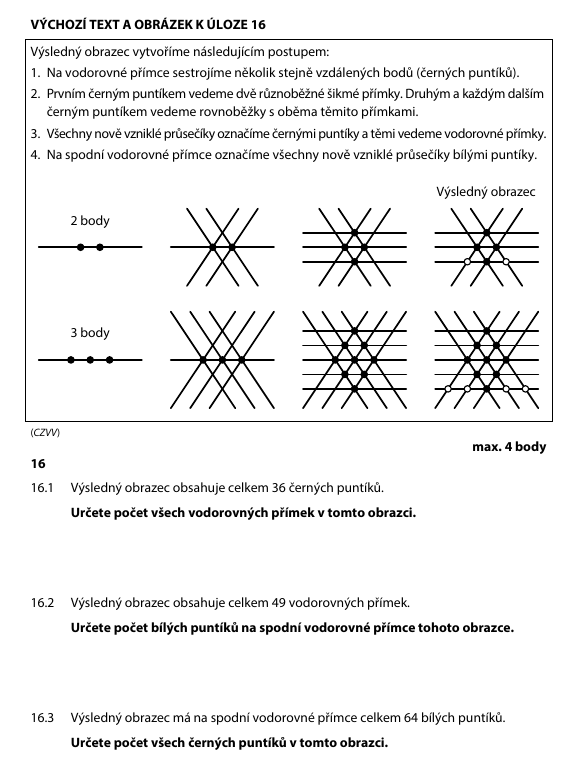
\includegraphics[width=0.6\textwidth]{opakujici_se_uloha}
\end{figure}


\section{Tvorba úloh vlastní sbírky}

Pro vlastní sbírku jsme se rozhodli tvořit úlohy pro 8leté obory. Bylo to zčásti kvůli typu úloh které obsahují, a zčásti kvůli tomu že sám studuji 8letý obor.

Úlohy jsme vytvářeli podle poznámek. Často jsou vysoce inspirované úlohami, které se v pravých zkouškách objevily.

Tvořené úlohy se liší od úloh CERMAT hlavně vzhledem, který je barevný, veselejší a přehlednější, a tím, že formát odpovědi tvořených úloh je otevřený. Student tak nemá na výběr z určitých možností a nemůže si tak tipovat.

Úlohy CERMAT mají často na výběr z odpovědí A-E, nejspíš proto že se pak dají jednodušeji opravovat.

Další rozdíl je využití geometrického zápisu, které CERMAT nevyužívá. Pro jistotu se před sbírkou vyskytuje přehled vysvětlující co která značka znamená.

Úlohy jsou tvořeny v programu GeoGebra. Z něj jsou exportovány do formátu PDF a vloženy do sbírky. Stereometrické úlohy jsou exportovány do formátu PNG, jelikož 3d GeoGebra nepodporuje ani PDF ani jiné vektorové formáty.
